\documentclass[border=1in]{standalone}
\usepackage{tikz}
\usetikzlibrary{arrows, math}

% ensures a white background in the converted image
\pagecolor{white}

\begin{document}
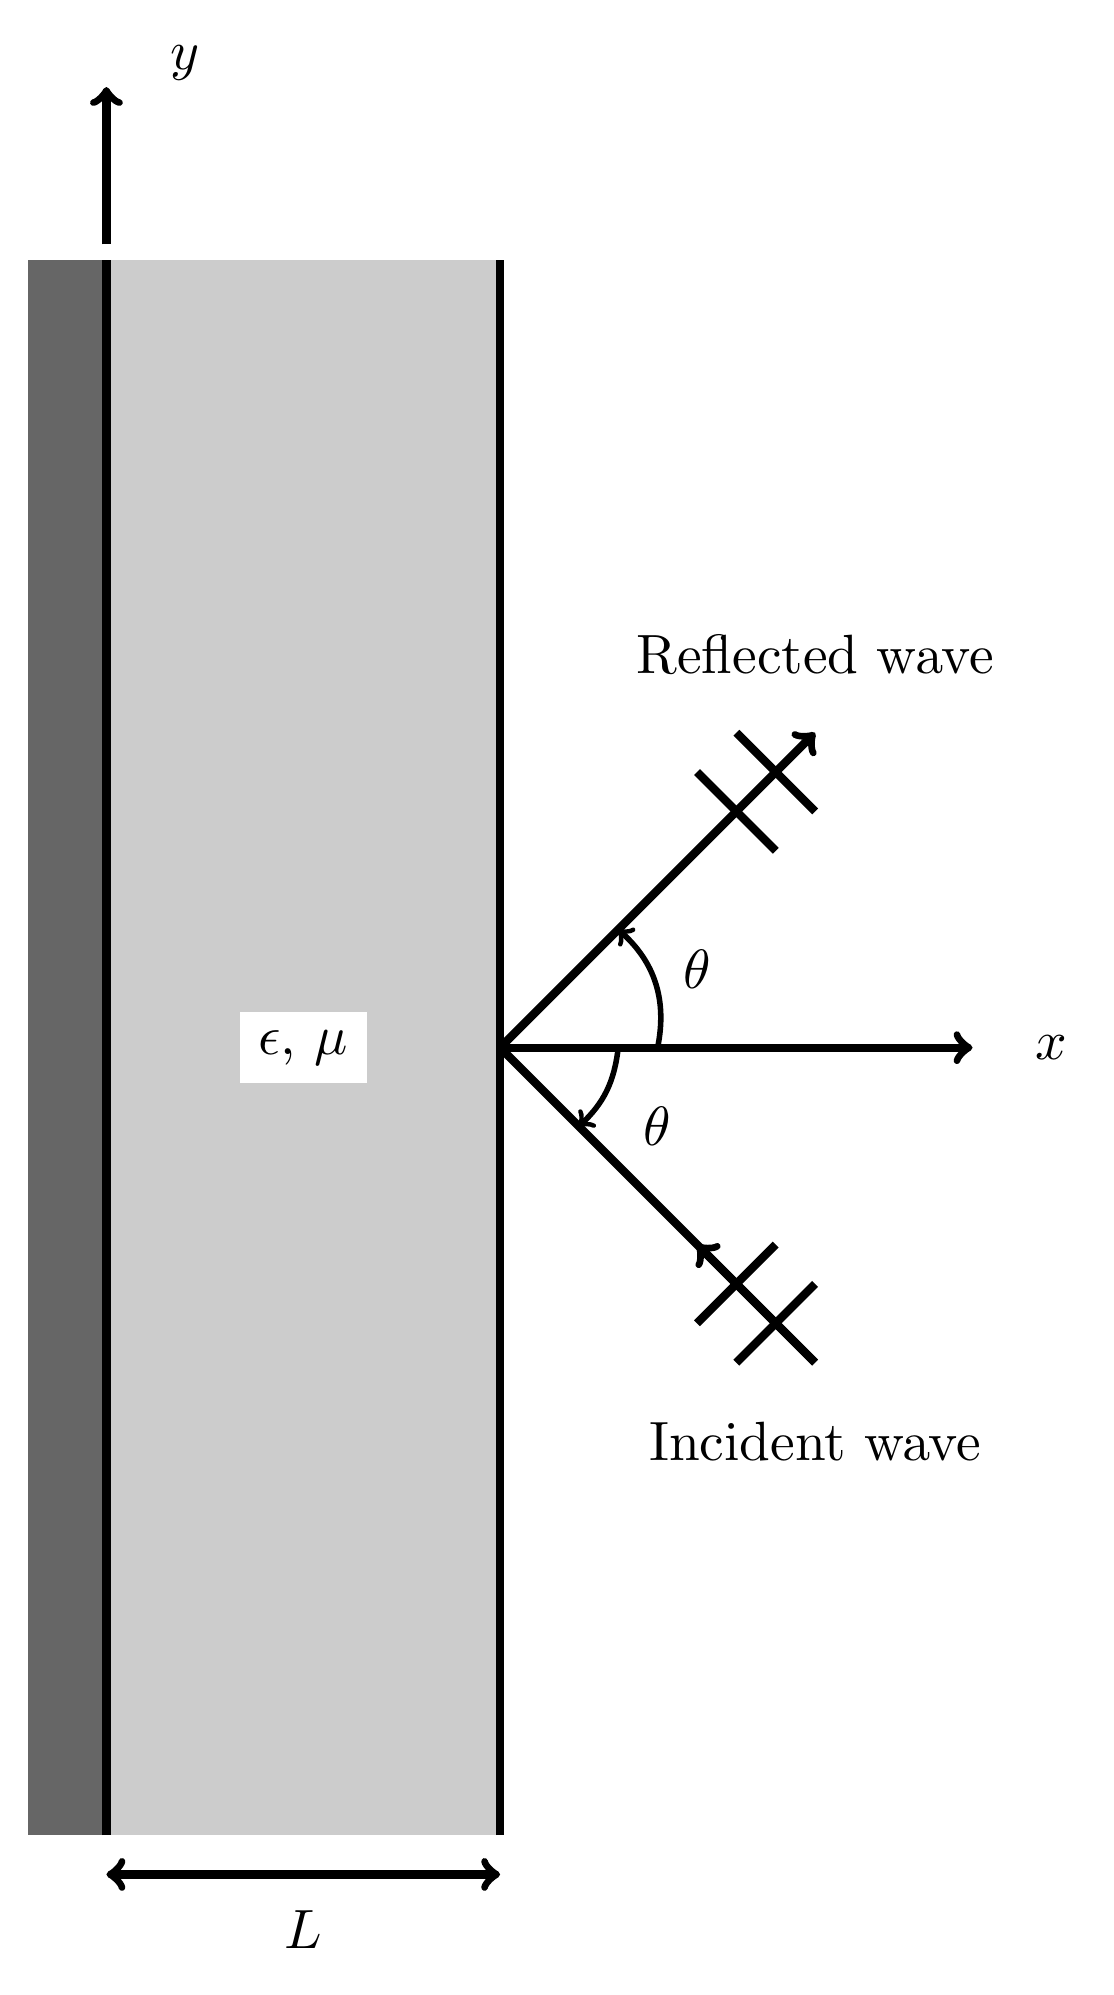
\begin{tikzpicture}
  % draw fills so lines sit on top of them
  \fill [fill=black!60!white] (0, 0) rectangle (1, 20);
  \fill [fill=black!20!white] (1, 0) rectangle (6, 20);
  % Draw lines
  \draw [line width=3pt] (1, 0) -- (1, 20);
  \draw [line width=3pt] (6, 0) -- (6, 20);
  % Draw width and axes arrows
  \draw[arrows=<->, line width=3pt] (1, -0.5) -- (6, -0.5);
  \draw[arrows=->, line width=3pt] (1, 20.2) -- (1, 22.2);
  \draw[arrows=->, line width=3pt] (6, 10) -- (12, 10);
  % Draw wave arrows and lines
  \draw[arrows=->, line width=3pt] (6, 10) -- (10, 14);
  \draw[line width=3pt] (10, 13) -- (9, 14);
  \draw[line width=3pt] (9.5, 12.5) -- (8.5, 13.5);
  \draw[line width=3pt] (10, 6) -- (6, 10);
  \draw[arrows=->, line width=3pt] (10, 6) -- (8.5, 7.5);
  \draw[line width=3pt] (9, 6) -- (10, 7);
  \draw[line width=3pt] (8.5, 6.5) -- (9.5, 7.5);
  % Draw angles
  \draw [arrows=->, line width=2pt] (8, 10) to [bend right=30] (7.5, 11.5);
  \draw [arrows=->, line width=2pt] (7.5, 10) to [bend left=20] (7, 9);
  % Add labels
  \node [fill=white, scale=2] at (2, 22.5) {$y$};
  \node [fill=white, scale=2] at (3.5, -1.2) {$L$};
  \node [fill=white, scale=2] at (3.5, 10) {$\epsilon$, $\mu$};
  \node [fill=white, scale=2] at (13, 10) {$x$};
  \node [fill=white, scale=2] at (8.5, 11) {$\theta$};
  \node [fill=white, scale=2] at (8, 9) {$\theta$};
  \node [fill=white, scale=2] at (10, 15) {Reflected wave};
  \node [fill=white, scale=2] at (10, 5) {Incident wave};
\end{tikzpicture}
\end{document}
